%===================================== CHAP 7 =================================
\chapter{Results}


\section{MiBots}
\section{Calibration }
\section{MB25}
\begin{table}[!h]
\begin{center}
\begin{tabular}{ | l | l | l | l |}
\hline
\textbf{Contact Spacing}&\textbf{200 \si{\micro \meter}} & \textbf{100 \si{\micro \meter}} & \textbf{50 \si{\micro \meter}} \\ \hline
\textbf{Average Resistivity (\si{\ohm - \cm})}&$0.0139$& $.0198$&$.0390$\\\hline
\textbf{Corrected Resistivity(\si{\ohm - \cm})}&0$.0122$& $0,0102$ &$.0101$\\\hline
\end{tabular}
\end{center}
\caption{Borate Si Fiber MB25. The correction factor is calculated from \cite{Zimney2007CorrectionStudy} with the assumption of a contact resistivity much greater than the core material. Considering the ratio of the measured resistance of the two point measurements compared to four point $\frac{.3}{50} = 150 $ this is a reasonable assumption.}
\label{Tabmb25}
\end{table}

The results in Table \ref{Tabmb25} shows the value of using multiple contacts to characterize a fiber, as there is good agreement in the measurements despite large deviations in the fiber diameter. It is hard to fit error bars considering the inhomogenity of the fiber, the designation of a core diameter as an average of the diameter at the ends is a somewhat arbitrary choice, and this introduces a systematic bias into the measurements. This also introduces error into the correction factors, as the ratio of contact spacing to diameter is what determines this value. This is a possibility, considering the $20\%$ difference in the uncorrected value as compared to the corrected values, be these correction factors are also derived for the case of a. 

\begin{figure}
    \centering
    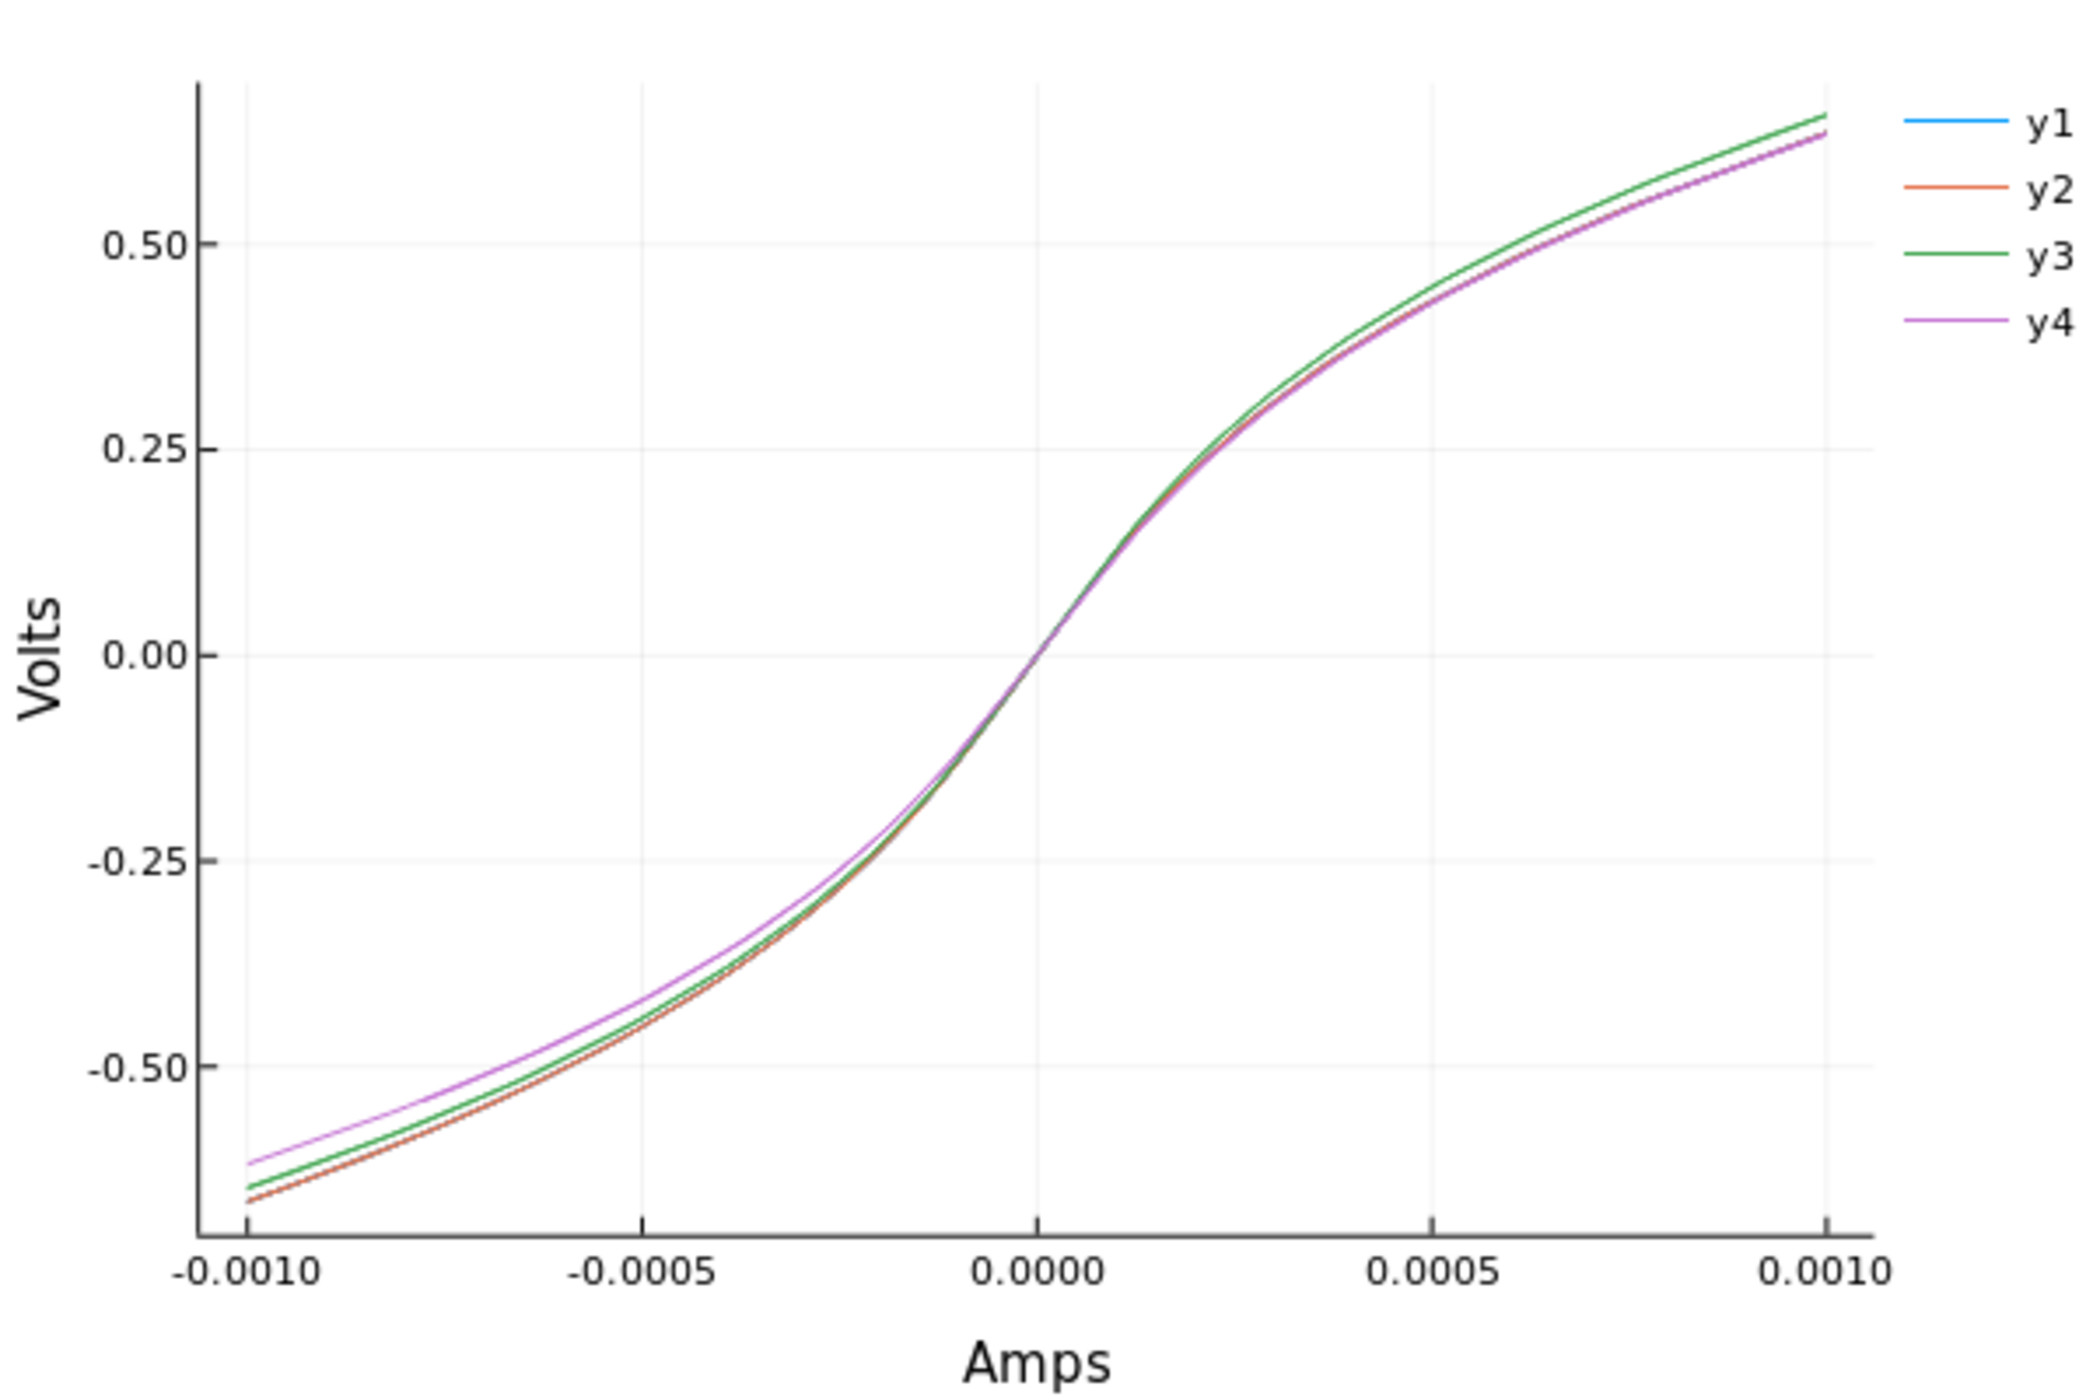
\includegraphics[width=\textwidth]{fig/Results/2pnt_compareMb25.jpg}
    \caption{}
    \label{fig:mb25 2pnt}
\end{figure}

While the resistance is nonohmic, fitting a line to the two-probe values, gives some idea of the similarity of the measurements. These values are $761, 739, 775, 755$. This could be considered an average resistivity in units of $\si{\ohm}$, but it is more clear to simply show that the contacts are similar to a reasonable degree. Plotting the values closer to 1 mA shows a resistance of $\sim 50 \si{\ohm}$  

This resistance includes the resistance of the Mibot probes, an interface resistance, and the resistance of the thin film. To isolate the contact resistance these can be subtracted from the measurement. The probe resistance is given by the manufacturer as:. Tuching the probe tips together and measuring the resistance gives a value of $\sim 10 \si{\ohm}$. Placing the probes on the same gold contact pad gives a value of$\sim 30$ therefore the majority of the resistance can be contributed to the contact resistance. Considering the sample preparation process is dirty by semiconductor manufacturing standards this is not surprising. It is standard procedure in industry to etch with Hydroflouric Acid before processing a silicon wafer.  Along with a native oxide layer, there is likely additional contamination from the lithography process, if no plasma cleaning is used after development of the resist. Visible contamination was observed with excess development therefore some contamination can be expected even when it is not directly visible.. This can be an explanation for the variance in contact resistivity, as a native oxide should be homogeneous across the fairy large contact pads. Another explanation is  poor adhesion of the contacts with the actual contact composed of smaller micro-contacts within the larger contact area, as observed in (). Sputtering is known to provide better adhesion, and it would be worth seeing if improvements in repeatability and resistance were found with sputtering over evaporation. Practically, this was not easy in the shared facilities at nanolab as a special request would be needed to have these materials installed as sputter targets in the instrument. 
 


\subsection{DB30618}


\begin{figure}
    \centering
    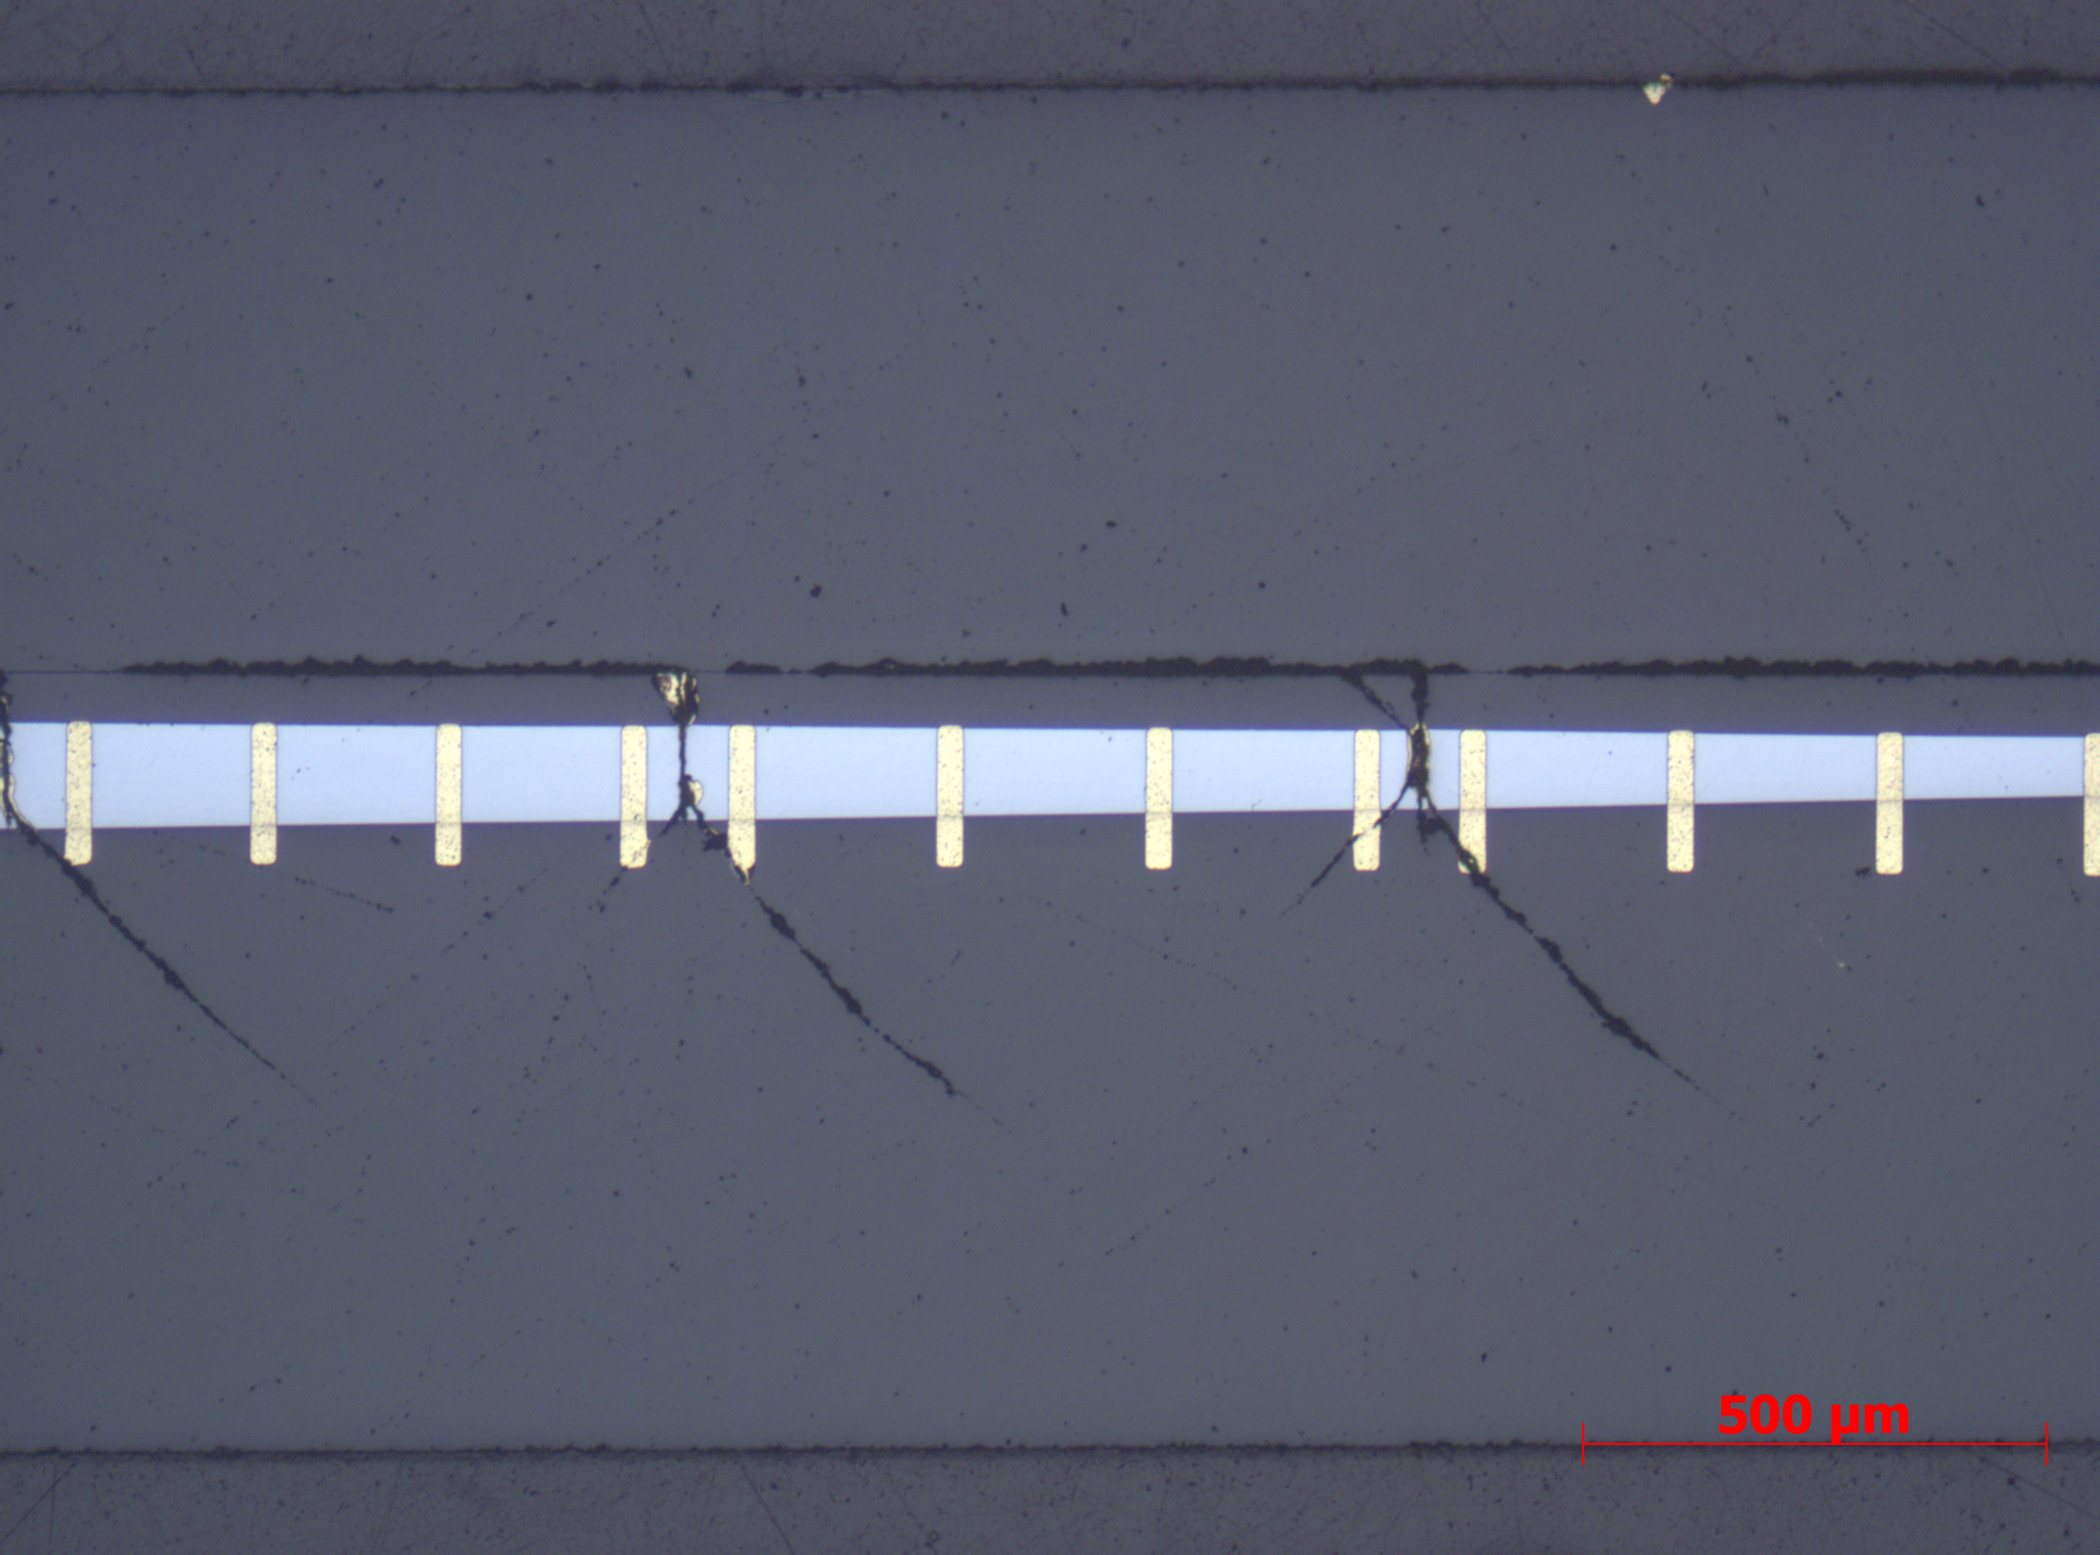
\includegraphics[width=\textwidth]{fig/Results/kthdb30618-8.jpg}
    \caption{Polished fiber: Db30618-8 KTH with deposited Au contacts for measurement with MiBot micro manipulators. The use of the MiBots allows measurement of the fiber, which would not have been possible with larger contact pads due to the cracks in the glass. It is also possible to make more measurements per sample as the larger contact pads have a 1mm spacing, and thus only 4-6 pads can be used on each side of the sample}
    \label{fig:db30618KTH}
\end{figure}


\begin{table}[!h]
\begin{center}
\begin{tabular}{ | l | l | l | l |}
\hline
\textbf{Sample}& DB30618-8 KTH & DB30618-6 NTNU \\ \hline
\textbf{Core Diameter}& $157-162$ & 40-46 \\\hline
\textbf{Number of locations}& 3&1 \\\hline
\textbf{Standard Deviation}& $0.0045$& NA \\\hline
\textbf{Averaged Resistivity $\si{\ohm-\cm}$}&$0.127 \pm 0.005$& $0.16 \pm .03$  \\\hline
\end{tabular}
\end{center}
\caption{The standard deviation shows. The error given is approximate, and calculated by calculating the resistivity for the largest and smallest core diameters. The contact was non-linear under one bias for DB30618-6 SH and thus only the linear half was considered. }
\label{Tabmb25}
\end{table}

\section{Db30418}
\begin{table}[!h]
\begin{center}
\begin{tabular}{ | l | l | l | l |}
\hline
\textbf{Sample}& DB30418-3 KTH & DB30418-3 NTNU \\ \hline
\textbf{Core Diameter $\si{\micro \meter}$}& $ 163-164.5$ & $28-40$ \\\hline
\textbf{Number of locations}&$3$&$2$ \\\hline
\textbf{Standard Deviation}& $\SI{1.75e-5}{\ohm \cm}$ & $ \SI{1.5e-5}{\ohm\cm}$ \\\hline
\textbf{Averaged Resistivity $\si{\ohm \cm}$}& $\SI{0.00061}{}\pm\SI{ 0.00002}{\ohm \cm}$ &$0.00072 \pm 0.0003 $ \\\hline
\end{tabular}
\end{center}
\caption{The standard deviation shows. The error given is approximate, and calculated by calculating the resistivity for the largest and smallest core diameters. The contact was non-linear under one bias for DB30618-6 SH and thus only the linear half was considered. }
\label{Tabmb25}
\end{table}





\begin{figure}[h]
 %h here H requires float, exactly here, h! overide latex
\centering
\begin{subfigure}{\textwidth}
  \centering
  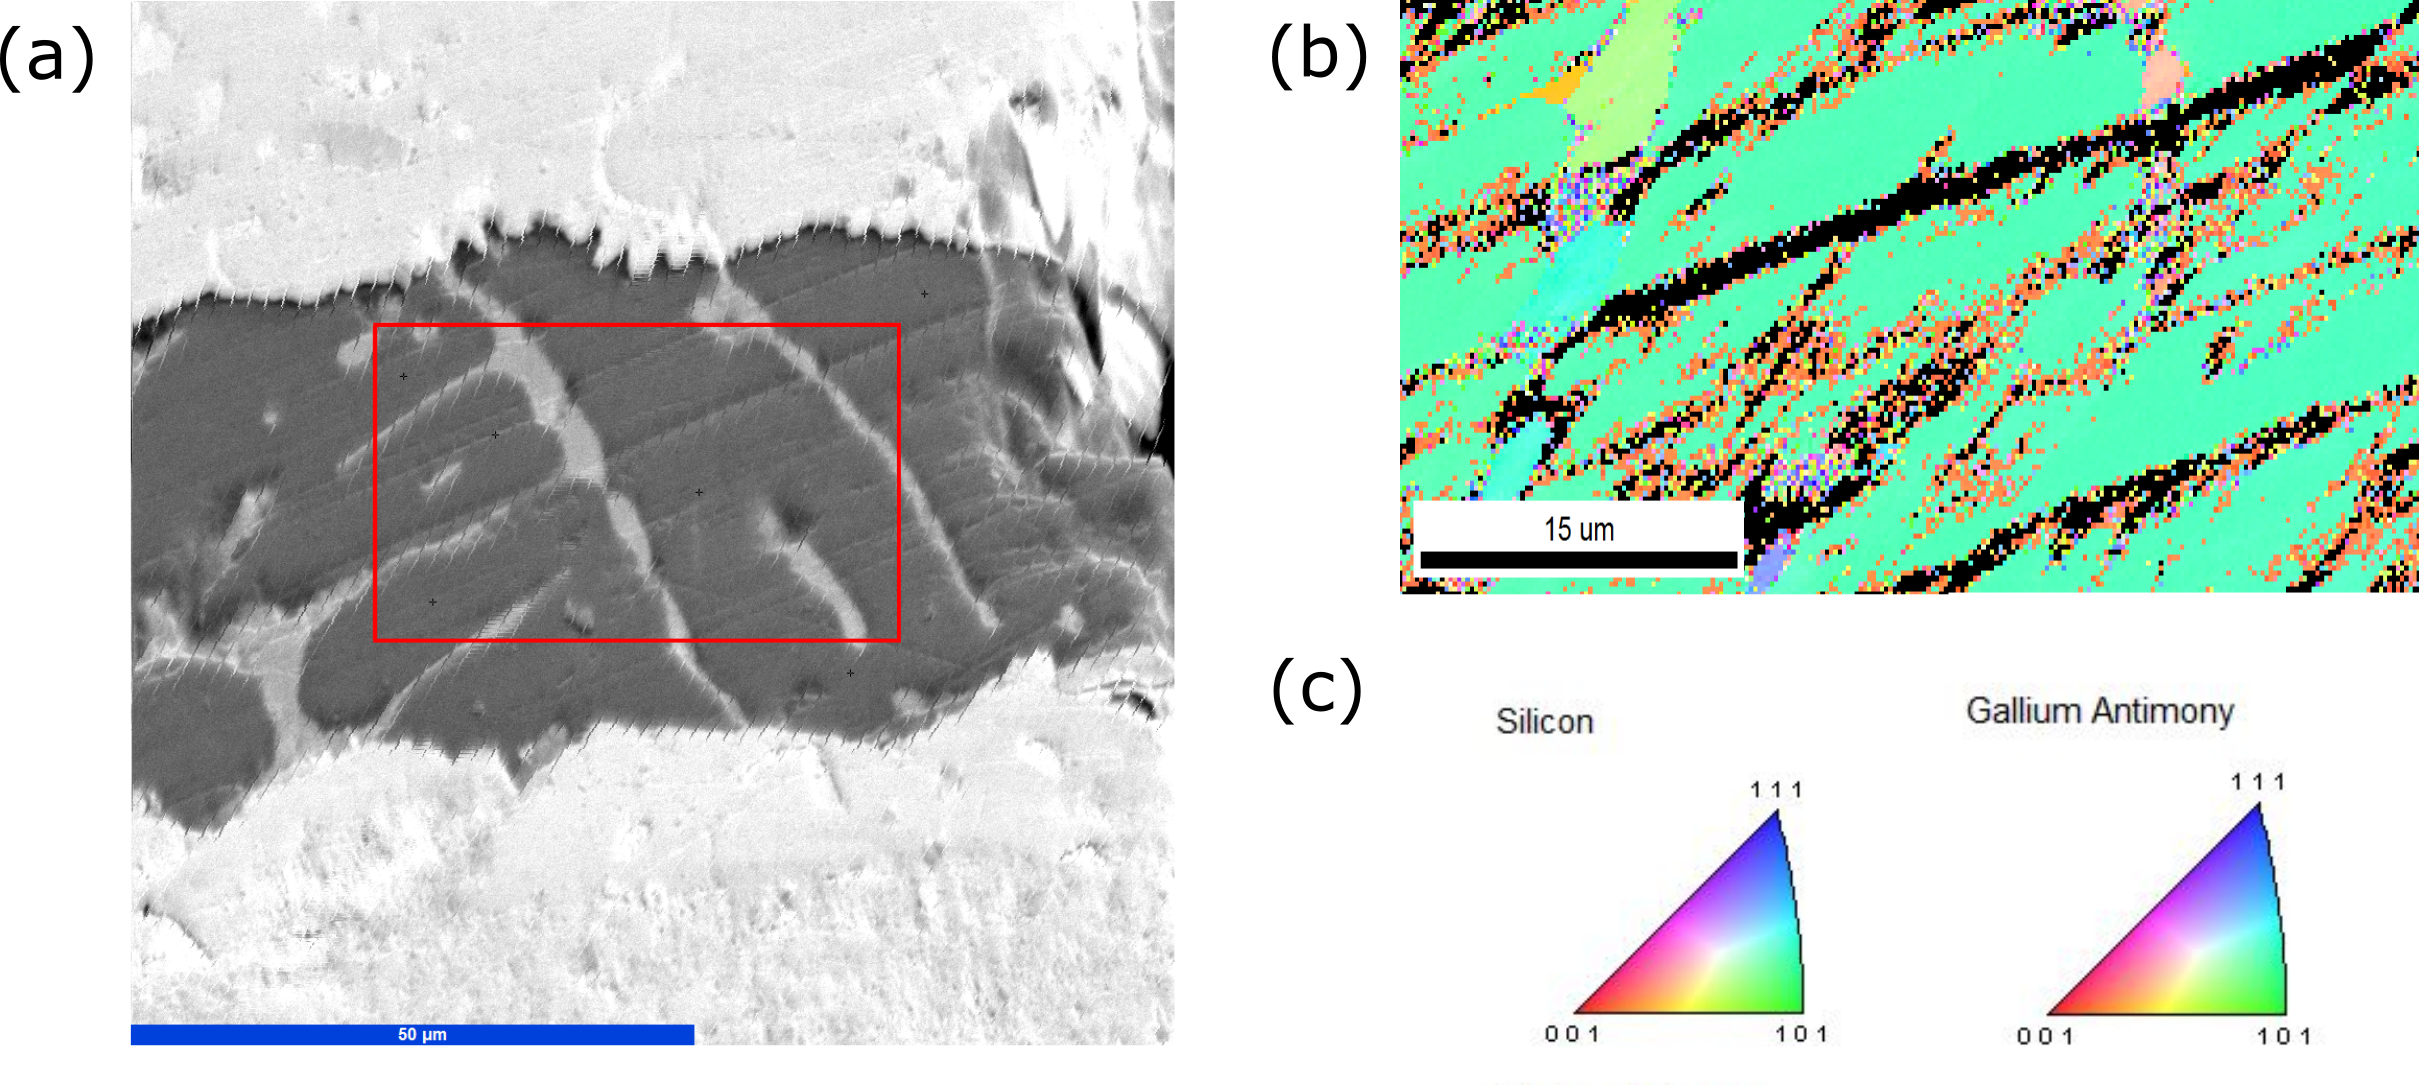
\includegraphics[width=\linewidth]{fig/ebsd.png}
  %\caption{1a}
  \label{fig:sfig1}
\end{subfigure}% %blank line makes figures vertical

\begin{subfigure}{\textwidth}
  \centering
  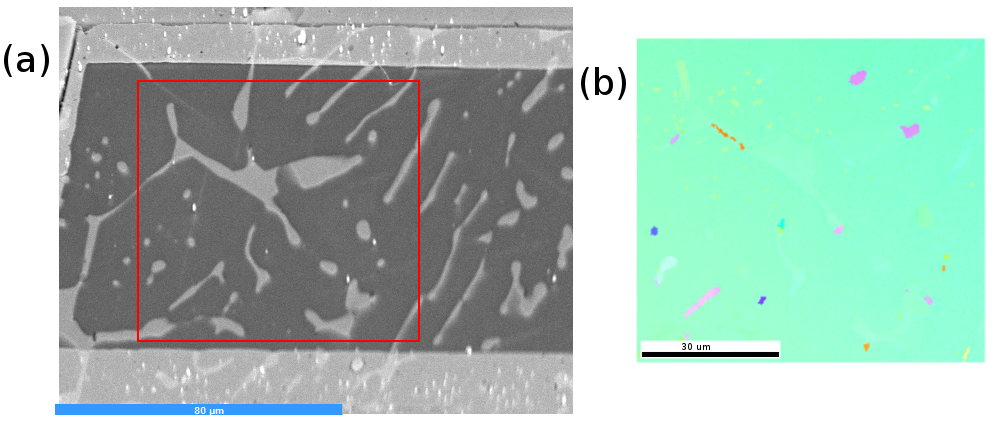
\includegraphics[width=\linewidth]{fig/ebsd_machinepolish.png}
  %\caption{1a}
  \label{fig:sfig2}
\end{subfigure}% %blank line makes figures vertical

\caption{}
\label{fig:ebsd}
\end{figure}


\section{Discussion}
Conclusions
The combination of mechanical polishing of an epoxy embedded fiber for use in Maskless Lithography, is promising for characterization of Semiconductor core fibers. The planar dimensions of the sample allow for integration with the existing instruments, which are primarily designed around the use of planar silicon wafers.  Maskless lithography provides more than sufficient resolution at the microscale. It allows for the mask design to be adapted to the changing fiber dimensions without creating a new physical chromium exposure mask, or shadow mask. Further the high resolution of the instrument allows for allignment with micrometer size features on the fiber which can allow for the measurement of specific junctions written in the fiber or areas of interest, as in the graded SiGe fibers produced in the group. The highest concentration areas being only several micrometers in length. The effects of strain in the fibers needs to be addressed in order to minimize cracking effects which are an obstacle to performing hall measurements. The use of micro manipulators provides of means of achieving a high number of measurement per fiber, which can lead to greater accuracy in resistivity meaurements. So far the measurements are limited to low resistivity materials. Annealing of contacts would not only open the range to accurate measurements of higher resistivity materials, but would open the possibility of additional measurement techniques () using one ohmic and one non ohmic contact. 
